\section{Wavelet}

 \begin{comment}
Il processo di convertire un segnale dal dominio del tempo a dom delle frequenze viene fatto tramite la trasformatadi Fourier (FT). Però Fourier non fornisce informazioni sufficienti su segnali non stazionari. FT determina soltanto le componenti di frequenza di un segnale, ma non la loro posizione nel tempo. Per risolvere questo inconveniente di usa STFT che usa una tecnica di “finestraggio”.
STFT associa il segnale in uno spazio bidimensionale di tempo e di frequenza utilizzando una singola finestra fissa.
Trasformata wavelet consente l'analisi con durate finestre multiple che consentono una prospettiva grossolana a multirisoluzione fine del segnale.
Essere in grado di dilatare o comprimere la regione variabile della finestra di dimensioni (wavelet), diverse caratteristiche del segnale saranno estratte in WT.
\end{comment}
Il processo di convertire un segnale dal dominio del tempo a dominio delle frequenze viene fatto tramite la trasformata di Fourier, per\`o Fourier non fornisce informazioni sufficienti su segnali non stazionari in quanto determina soltanto le componenti di frequenza di un segnale, ma non la loro posizione nel tempo.
La trasformata Wavelet consente un' analisi migliore per questo tipo di segnali. 

Una wavelet \`e una forma d'onda oscillante di lunghezza finita, con un ampiezza che parte da zero e aumenta e decrementa tornando a zero.
Al contrario delle sinusoidi usate nella trasformata di Fourier, le wavelet sono pi\`u concentrate nel tempo. 
Di solito forniscono una anailsi del segnale che \`e localizzato sia nel tempo che nella frequenza mentre la trasformata di Fourier \`e localizzata solo nella frequenza. 
Un esempio di wavelet \`e rappresentato dalla figura seguente:
\begin{comment}
\begin{figure}[h]
 \centering
 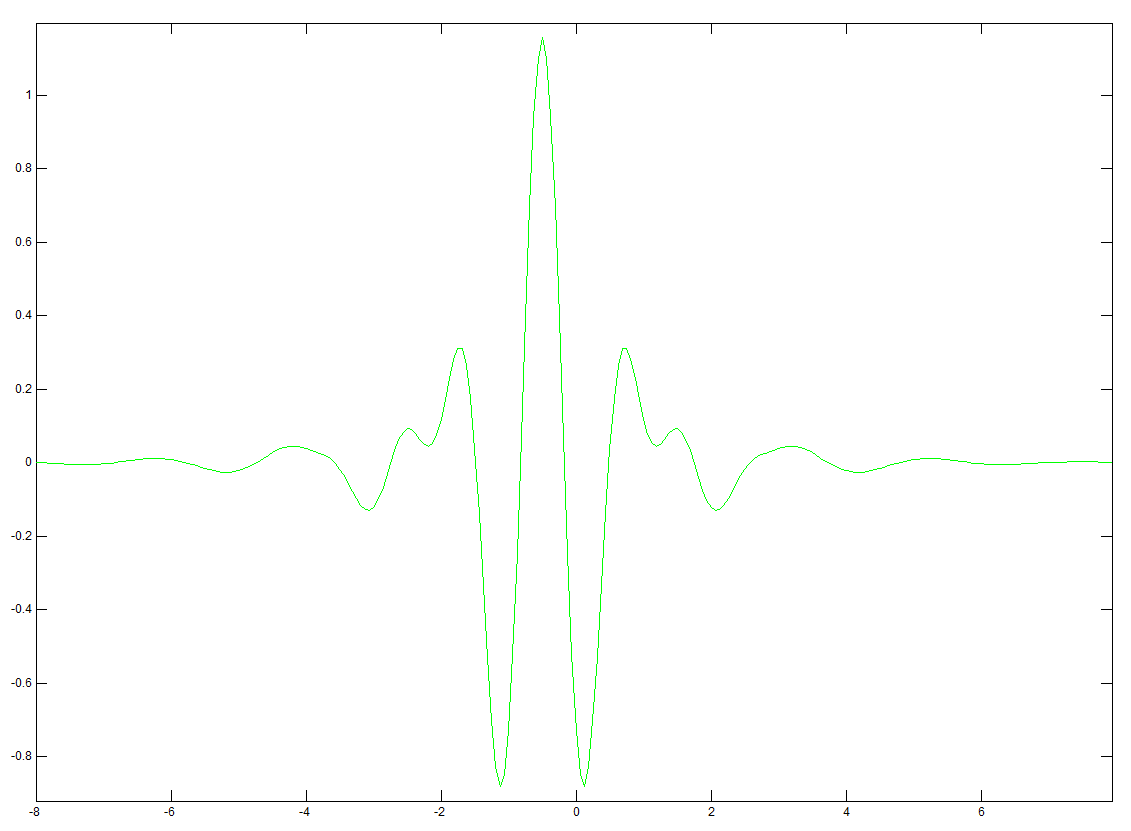
\includegraphics[width=0.4\textwidth]{./Meyerwavelet.png}
 % Meyerwavelet.png: 1131x831 pixel, 72dpi, 39.90x29.32 cm, bb=0 0 1131 831
 \label{fig: Meyer wavelet}
\end{figure}
\end{comment}


Una funzione $\psi(t)$ \`e una wavelet se soddisfa i seguenti criteri:
\begin{itemize}
  \item 
    Una wavelet deve avere energia finita.
    \[
      E=\displaystyle \int_{-\infty}^{\infty} |\psi(t)|^{2} dt < \infty
    \]
  \item
    Se $\Psi$ \`e la trasformata di Fourier della wavelet $\psi(t)$ allora $\Psi(0)=0$. Cio\`e la wavelet non ha componenti nella frequenza zero.
  \item
    La trasformata di Fourier di una wavelet complessa deve essere reale e deve essere nulla nelle frequenze negative.
\end{itemize}

\section{Trasformata wavelet continua}
Sia $\psi(t)$ una wavelet, definiamo la trasformata wavelet continua di una funzione $x(t)$ come 
\[
  X(a,b)=\displaystyle \frac{1}{\sqrt{a}}\displaystyle\int_{-\infty}^{\infty} \psi \left( \frac{t-b}{a} \right) x(t) dt
\]

La scala o parametro di dilatazione $a$ corrisponde all'informazione di frequenza e il parametro di traslazione $b$ si riferisce alla locazione della funzione wavelet mentre viene fatta spostare lungo il segnale quindi corrisponde all'informazione temporale nella trasformata.
%Ci sono molte scelte per la wavelet madre.
Esiste anche la trasformata wavelet discreta che opera su segnali a tempo discreto e che restituisce coefficienti discreti nel dominio delle wavelet.
I parametri $a$ e $b$ assumono valori in una griglia discreta
\[
  \begin{array}{llll}
      a=2^{-j}
    &
      b=k\cdot 2^{-j}
    &
     
    &
      j,k\in \mathbb{Z}
  \end{array}
\]


\cite{wavelet1}\cite{wavelet2}
